\subsection{Understand your purpose}

It is important to have a clear idea of why you are publishing your data. Most of the principles
we describe are applicable to both commercial concerns i.e. you have some data that you think
people will pay for, and public-good data, such as in our Aire Guru website. We write, however,
with the assumption that you want to maximise your attraction to your users, who are most likely
the general public, or some subset thereof, and who are not scientifically motivated.\\

A significant difference between public-good and commercial offerings is that the former are usually
unique with respect to your target market. So if similar data is already available, it is likely technically
inferior in some objective respect. Maybe you have more up-to-date or accurate data,
greater coverage of information, or unique functionality that is not currently offered e.g. a way of using the
information you provide to solve a daily problem.\\

A commercial offering on the other hand, might have to compete on
non-technical aspects to get users. The rest of this section focuses on public-good offerings. \\

Once our purpose is defined, we face a series of problems; the user may not even be aware of the value of our data.
Thus we have a double challenge, to deliver the data, and to convince the user that it is really necessary, that it can help them in their routine or daily life.\\

Reaching users is only the beginning of the relationship - we want them to remain with us.
We need to earn their trust. We need them to values us, appreciate us, feel a connection with us.
We have to cultivate the relationship, look after our users and provide continual satisfaction.\\

This is where we can make use of the most appropriate marketing techniques to reach our users.
We will have to conduct a study of our target audience, find out what type of advertising they consume and through which channels,
so we can approach them in the most appropriate way. Today's market is in a fast paced state of continuous change,
so we must be flexible and adapt to find the perfect formula. \\

\subsubsection*{Suggested strategies}

\begin{itemize}
    \item Study and analyze what the current gaps in the market are, and what needs the user might have that aren't being met.
    \item Define your target audience. What do they use in their daily life to keep informed or for entertainment?
    What type of advertising do they already consume? How can we get closer to them?
    \item Keep in mind that we must stay faithful to the spirit of what we represent, so as well as understanding what advertising fits the user,
    we should know what kind of advertising adapts most suitably to our product.
\end{itemize}

\subsubsection*{In the context of Aire Guru \ldots}

The goal of Aire Guru is to increase the awareness of the quality of the air.
There are several problems regarding this issue, the first one is user ignorance.
Users are generally not aware of the actual levels of pollution to which they are exposed, and most do not know how such pollution can harm them,
both in the short and long terms.\\

Aire Guru shows how air quality influences us, in a way that everyone, independent of their cultural or educational level, can clearly understand.
It aims to make the information, and what that information means, available to everyone.
We show how harmful it is to live in a highly polluted area and what the most common sources of pollution
are, so that we can increase awareness and empower users to do something about it.\\

Aire Guru includes in its glossary the most common medical conditions that may be affected by air pollution, the pollutants, and the sources that produce these pollutants.
It is accompanied by an iconography which reflects each of the symptoms. \\

In a survey conducted after launch, users told us that their interest in air pollution had grown.
Some of them discovered that they had a medical condition that is affected by the pollution.\\

\begin{figure}[ht]
    \centering
    \subfigure[Glossary detail]
        {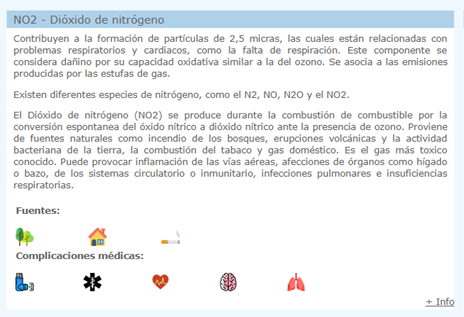
\includegraphics[width=6.2cm]{no2_glosary}}
    \hfill
    \subfigure[Iconography detail]
        {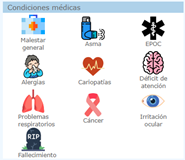
\includegraphics[width=5cm]{iconography}}
    \caption{Glossary}
\end{figure}